\documentclass[a4paper,10pt,twoside,final,spanish]{article}

% Preámbulo - Parte A

\usepackage[utf8]{inputenc} % Soporte para los acentos
\usepackage[T1]{fontenc}

\usepackage[spanish]{babel} % Capítulos, seciones, etc. en español

\usepackage[margin=2cm]{geometry} % Diseño del documento

\usepackage{multicol} % Escribir doble columna

\usepackage{xcolor} % Usar colores
\usepackage{pstricks}

\usepackage{enumerate} % Cambiar etiquetas de numeración
\usepackage[shortlabels]{enumitem} % Manejo adicional de etiquetas de numeración

\usepackage{graphicx} % Manejo de gráficos y figuras

\usepackage{makeidx} % Índice alfabético

% Paquetes adicionales de símbolos matemáticos
\usepackage{amsmath,amssymb,amsfonts,latexsym} 

% \usepackage{pslatex} % Fuente Times
% \usepackage{mathpazo} % Fuente Palatino
% \usepackage{mathptmx} % Fuente Times
% \usepackage{bookman} % Fuente Bookman
% \usepackage{newcent} % Fuente New Century Schoolbook
% \usepackage{helvet} % Fuente Helvetica
 \usepackage{palatino} % Fuente Palatino
% \usepackage{pxfonts} % Fuente 
% \usepackage{txfonts} % Fuente
% \usepackage{concrete} % Fuente
% \usepackage{cmbright} % Fuente
% \usepackage{fourier} % Fuente

\usepackage{booktabs} % Opciones adicionales para el entorno tabular
\usepackage{longtable} % Para tablas de más de una página

\usepackage{tikz} % Creación de gráficos

\usepackage{hyperref}

\usepackage{textcomp}
\usepackage{gensymb} %para los grados celcius
\usepackage[makeroom]{cancel} %Para tachar expresiones matemáticas
\newcommand\Ccancel[2][black]{\renewcommand\CancelColor{\color{#1}}\cancel{#2}}

\usepackage{soul} % para tachar texto
\pagestyle{headings}
% Para encerrar expresiones con círculos
\usepackage{mathtools}% superior to amsmath
\usepackage{siunitx} % para escribir grados minutos segundos
\usepackage{tikz}
\makeatletter
\newcommand\mathcircled[1]{%
  \mathpalette\@mathcircled{#1}%
}
\newcommand\@mathcircled[2]{%
  \tikz[baseline=(math.base)] \node[draw,circle,inner sep=1pt] (math) {$\m@th#1#2$};%
}
\makeatother
%---
\usepackage{fancyhdr} %Para usar encabezados y pies personalizados
	\pagestyle{fancy}
	\fancyhf{}
	\fancyhead[LE,RO]{Mecánica del Continuo}
	\fancyhead[RE,LO]{Análisis de Deformación}
	\fancyfoot[LE,RO]{\thepage}
	\fancyfoot[RE,LO]{Darién Julián Ramírez}	
	\renewcommand{\footrulewidth}{1pt}
%---
\usepackage{listings} %Para escribir códigos
\lstset{language=XML,
	basicstyle=\footnotesize,
	numbers=left,
 	stepnumber=1,
	numbersep=8pt,
	showspaces=false,               % show spaces adding particular underscores
  	showstringspaces=false,         % underline spaces within strings
  	frame=lines,                   % adds a frame around the code
	tabsize=4,                      
  	captionpos=b,                   % sets the caption-position to bottom
  	breaklines=true,                % sets automatic line breaking
}
%---

% Preámbulo - Parte B

\title{\Huge Mecánica del Continuo \\
			 Trabajo Práctico Nº5  \\
			 Análisis de Deformación}
\author{Darién Julián Ramírez}
\date{}

% Cuerpo del documento

\begin{document}

\maketitle % Mostrar título

\section*{Ejercicio 1}

Considerar una placa cuadrada de tamaño unitario como la que se observa en la figura \ref{fig:ej1}. 
Determinar las componentes de deformación. 

\begin{figure}[htbp]
\centerline{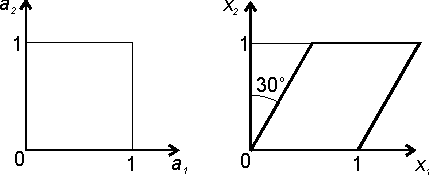
\includegraphics[scale=1.25]{ej1}}
\caption{Placa cuadrada de tamaño unitario.}
\label{fig:ej1}
\end{figure}

\dotfill

\begin{quote}

\[
\tan 30\degree=\tan\left(\frac{\pi}{6}\right)
=\frac{\sin\left(\frac{\pi}{6}\right)}{\cos\left(\frac{\pi}{6}\right)}
=\frac{\frac{1}{2}}{\frac{\sqrt{3}}{2}}=\frac{1}{\sqrt{3}}\frac{\sqrt{3}}{\sqrt{3}}
=\frac{\sqrt{3}}{3}
\]

\[
\begin{array}{rcl}
\mbox{original}(a_{1},a_{2}) &     & \mbox{deformado}(x_{1},x_{2})  \\
(0,0)                        & \to & (0,0)                          \\
(1,0)                        & \to & (1,0)                          \\
(0,1)                        & \to & (0+1\cdot\frac{\sqrt{3}}{3},1) \\
(1,1)                        & \to & (1+1\cdot\frac{\sqrt{3}}{3},1)
\end{array}
\]

Enfoque Lagrangiano:

\[
\begin{array}{ccc}
x_{i}=x_{i}(a_{1},a_{2}) & \implies & \left\{\begin{array}{l}
 								   x_{1}(a_{1},a_{2})=a_{1}+\frac{\sqrt{3}}{3}a_{2} \\
   								   x_{2}(a_{1},a_{2})=a_{2}
   								   \end{array}\right.
\end{array}
\]

\textit{Tensor de deformación de Green:}

\[
E_{ij}=
\frac{1}{2}\left(
\frac{\partial x_{\alpha}}{\partial a_{i}}
\frac{\partial x_{\alpha}}{\partial a_{j}}-\delta_{ij}
\right)
\]

\begin{minipage}{0.5\linewidth}

\begin{align*}
E_{11} &=
\frac{1}{2}\left(
\frac{\partial x_{\alpha}}{\partial a_{1}}
\frac{\partial x_{\alpha}}{\partial a_{1}}-\delta_{11}
\right) \\
&=
\frac{1}{2}\left(
\left(\frac{\partial x_{\alpha}}{\partial a_{1}}\right)^{2}-1
\right) \\
&=
\frac{1}{2}\left(
\left(\frac{\partial x_{1}}{\partial a_{1}}\right)^{2}
+\left(\frac{\partial x_{2}}{\partial a_{1}}\right)^{2}-1
\right) \\
&=
\frac{1}{2}(1^{2}+0^{2}-1) \\
&= 0
\end{align*}

\end{minipage} \hfill \begin{minipage}{0.5\linewidth}

\begin{align*}
E_{22} &=
\frac{1}{2}\left(
\frac{\partial x_{\alpha}}{\partial a_{2}}
\frac{\partial x_{\alpha}}{\partial a_{2}}-\delta_{22}
\right) \\
&=
\frac{1}{2}\left(
\left(\frac{\partial x_{\alpha}}{\partial a_{2}}\right)^{2}-1
\right) \\
&=
\frac{1}{2}\left(
\left(\frac{\partial x_{1}}{\partial a_{2}}\right)^{2}
+\left(\frac{\partial x_{2}}{\partial a_{2}}\right)^{2}-1
\right) \\
&=
\frac{1}{2}\left(\left(\frac{\sqrt{3}}{3}\right)^{2}+1^{2}-1\right) \\
&= \frac{1}{6}
\end{align*}

\end{minipage}

\begin{minipage}{0.5\linewidth}

\begin{align*}
E_{12} &=
\frac{1}{2}\left(
\frac{\partial x_{\alpha}}{\partial a_{1}}
\frac{\partial x_{\alpha}}{\partial a_{2}}-\delta_{12}
\right) \\
&=
\frac{1}{2}\left(
\frac{\partial x_{1}}{\partial a_{1}}
\frac{\partial x_{1}}{\partial a_{2}}
+\frac{\partial x_{2}}{\partial a_{1}}
\frac{\partial x_{2}}{\partial a_{2}}
-0
\right) \\
&=
\frac{1}{2}\left(
1\cdot
\frac{\sqrt{3}}{3}
+0\cdot
1
\right) \\
&=
\frac{1}{2}\frac{\sqrt{3}}{3} \\
&=\frac{\sqrt{3}}{6}
\end{align*}

\end{minipage} \hfill \begin{minipage}{0.5\linewidth}

\[
\mathbf{E}=
\begin{pmatrix}
0                  & \frac{\sqrt{3}}{6} \\
\frac{\sqrt{3}}{6} & \frac{1}{6}
\end{pmatrix}
\]

\end{minipage} \\

Enfoque Euleriano:

\[
\begin{array}{ccc}
a_{i}=a_{i}(x_{1},x_{2}) & \implies & \left\{\begin{array}{l}
 								   a_{1}(x_{1},x_{2})=x_{1}-\frac{\sqrt{3}}{3}x_{2} \\
   								   a_{2}(x_{1},x_{2})=x_{2}
   								   \end{array}\right.
\end{array}
\]

\textit{Tensor de deformación de Almansi:}

\[
e_{ij}=
\frac{1}{2}\left(
\delta_{ij}-
\frac{\partial a_{\alpha}}{\partial x_{i}}
\frac{\partial a_{\alpha}}{\partial x_{j}}
\right)
\]

\begin{minipage}{0.5\linewidth}

\begin{align*}
e_{11} &=
\frac{1}{2}\left(\delta_{11}-
\frac{\partial a_{\alpha}}{\partial x_{1}}
\frac{\partial a_{\alpha}}{\partial x_{1}}
\right) \\
&=
\frac{1}{2}\left(1-
\left(\frac{\partial a_{\alpha}}{\partial x_{1}}\right)^{2}
\right) \\
&=
\frac{1}{2}\left(1-\left(
\left(\frac{\partial a_{1}}{\partial x_{1}}\right)^{2}
+\left(\frac{\partial a_{2}}{\partial x_{1}}\right)^{2}
\right)\right) \\
&=
\frac{1}{2}(1-1^{2}-0^{2}) \\
&=0
\end{align*}

\end{minipage} \hfill \begin{minipage}{0.5\linewidth}

\begin{align*}
e_{22} &=
\frac{1}{2}\left(\delta_{22}-
\frac{\partial a_{\alpha}}{\partial x_{2}}
\frac{\partial a_{\alpha}}{\partial x_{2}}
\right) \\
&=
\frac{1}{2}\left(1-
\left(\frac{\partial a_{\alpha}}{\partial x_{2}}\right)^{2}
\right) \\
&=
\frac{1}{2}\left(1-\left(
\left(\frac{\partial a_{1}}{\partial x_{2}}\right)^{2}
+\left(\frac{\partial a_{2}}{\partial x_{2}}\right)^{2}
\right)\right) \\
&=
\frac{1}{2}\left(1-\left(\frac{\sqrt{3}}{3}\right)^{2}-1^{2}\right) \\
&=-\frac{1}{6}
\end{align*}

\end{minipage}

\begin{minipage}{0.5\linewidth}

\begin{align*}
e_{12} &=
\frac{1}{2}\left(\delta_{12}-
\frac{\partial a_{\alpha}}{\partial x_{1}}
\frac{\partial a_{\alpha}}{\partial x_{2}}
\right) \\
&=
\frac{1}{2}\left(0-
\frac{\partial a_{1}}{\partial x_{1}}
\frac{\partial a_{1}}{\partial x_{2}}
-\frac{\partial a_{2}}{\partial x_{1}}
\frac{\partial a_{2}}{\partial x_{2}}
\right) \\
&=
\frac{1}{2}\left(
1\cdot
\frac{\sqrt{3}}{3}
-0\cdot
1
\right) \\
&=
\frac{1}{2}\frac{\sqrt{3}}{3} \\
&=\frac{\sqrt{3}}{6}
\end{align*}

\end{minipage} \hfill \begin{minipage}{0.5\linewidth}

\[
\mathbf{e}=
\begin{pmatrix}
0                  & \frac{\sqrt{3}}{6} \\
\frac{\sqrt{3}}{6} & -\frac{1}{6}
\end{pmatrix}
\]

\end{minipage}

\end{quote}

\section*{Ejercicio 2}

Considere la misma placa del ejercicio anterior (Figura \ref{fig:ej1}), pero esta vez sujeta a una distorsión mucho más pequeña definida por: 

\[
\begin{array}{cccc}
x_{1}=a_{1}+0.01a_{2}; &
a_{1}=x_{1}-0.01x_{2}; &
x_{2}=a_{2};           &
x_{3}=a_{3}
\end{array}
\]

Determine las componentes de deformación.

\dotfill

\begin{quote}
\textit{Tensor de deformación infinitesimal de Cauchy:}

\[
e_{ij}=\frac{1}{2}\left(
\frac{\partial u_{j}}{\partial a_{i}}+
\frac{\partial u_{i}}{\partial a_{j}}
\right)
=
\frac{1}{2}\left(
\frac{\partial u_{j}}{\partial x_{i}}+
\frac{\partial u_{i}}{\partial x_{j}}
\right)
\]

\begin{align*}
e_{11} &= \frac{1}{2}\left(
\frac{\partial u_{1}}{\partial a_{1}}+
\frac{\partial u_{1}}{\partial a_{1}}
\right)
=
\frac{\partial u_{1}}{\partial a_{1}}=0 &
u_{1} &= x_{1}-a_{1}=a_{1}+0.01a_{2}-a_{1}=0.01a_{2} \\
e_{22} &= \frac{1}{2}\left(
\frac{\partial u_{2}}{\partial a_{2}}+
\frac{\partial u_{2}}{\partial a_{2}}
\right)
=
\frac{\partial u_{2}}{\partial a_{2}}=0 &
u_{2} &= x_{2}-a_{2}=a_{2}-a_{2}=0 \\
e_{12} &= \frac{1}{2}\left(
\frac{\partial u_{2}}{\partial a_{1}}+
\frac{\partial u_{1}}{\partial a_{2}}
\right)
=
\frac{1}{2}\cdot0.01=0.005 &
\end{align*}

\[
\mathbf{e}=
\begin{pmatrix}
0 & 0.005 \\
0.005 & 0
\end{pmatrix}
\]

\begin{align*}
e_{11} &= \frac{1}{2}\left(
\frac{\partial u_{1}}{\partial x_{1}}+
\frac{\partial u_{1}}{\partial x_{1}}
\right)
=
\frac{\partial u_{1}}{\partial x_{1}}=0 &
u_{1} &= x_{1}-a_{1}=x_{1}-x_{1}+0.01x_{2}=0.01x_{2} \\
e_{22} &= \frac{1}{2}\left(
\frac{\partial u_{2}}{\partial x_{2}}+
\frac{\partial u_{2}}{\partial x_{2}}
\right)
=
\frac{\partial u_{2}}{\partial x_{2}}=0 &
u_{2} &= x_{2}-a_{2}=x_{2}-x_{2}=0 \\
e_{12} &= \frac{1}{2}\left(
\frac{\partial u_{2}}{\partial x_{1}}+
\frac{\partial u_{1}}{\partial x_{2}}
\right)
=
\frac{1}{2}\cdot0.01=0.005
\end{align*}

\[
\mathbf{e}=
\begin{pmatrix}
0 & 0.005 \\
0.005 & 0
\end{pmatrix}
\]
\end{quote}

\section*{Ejercicio 3}

Sea $ABCD$ un cuadrado unitario en el plano $xy$ (Figura \ref{fig:ej3}).

\begin{figure}[htbp]
\centerline{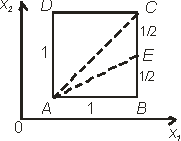
\includegraphics[scale=1.5]{ej3}}
\caption{Cuadrado unitario $ABCD$.}
\label{fig:ej3}
\end{figure}

$ABCD$ forma parte de un gran cuerpo deformable sujeto a una pequeña deformación uniforme dada por:

\[
e_{ij}=
\left(
\begin{matrix}
0.001 & 0.002 & 0.003 \\
0.002 & 0.001 & 0     \\
0.003 & 0     & 0.002
\end{matrix}
\right)
\]

¿Cuál es el cambio de longitud de las líneas $AC$ y $AE$?

\dotfill

\begin{quote}

\[
\begin{array}{rcll}
dS^{2}-dS_{0}^{2}          & = & 2e_{ij}dx_{i}dx_{j}; & 
dS^{2}-dS_{0}^{2}=(dS-dS_{0})(dS+dS_{0})\\
(dS-dS_{0})(dS+dS_{0})     & = & 2e_{ij}dx_{i}dx_{j}; & 
dS=dS_{0}\\
(dS-dS_{0})(dS_{0}+dS_{0}) & = & 2e_{ij}dx_{i}dx_{j} & \\
(dS-dS_{0})(2dS_{0})       & = & 2e_{ij}dx_{i}dx_{j} & \\[0.15cm]
dS-dS_{0}                  & = & \frac{2e_{ij}dx_{i}dx_{j}}{2dS_{0}} & \\[0.15cm]
dS-dS_{0}                  & = & \frac{e_{ij}dx_{i}dx_{j}}{dS_{0}} 
								 \frac{dS_{0}}{dS_{0}} & \\[0.15cm]
dS-dS_{0}                  & = & e_{ij}\frac{dx_{i}}{dS_{0}}
 									   \frac{dx_{j}}{dS_{0}}dS_{0}; & 
\frac{dx_{i}}{dS_{0}}=n_{i};\quad\frac{dx_{j}}{dS_{0}}=n_{j} \\[0.15cm] 
dl                         & = & e_{ij}n_{i}n_{j}dS_{0} & \\[0.15cm]
\int_{0}^{l}dl             & = & e_{ij}n_{i}n_{j}\int_{0}^{l}dS_{0} & \\[0.15cm]
\Delta l                   & = & e_{ij}n_{i}n_{j}l_{0}=n_{i}e_{ij}n_{j}l_{0} &
\end{array}
\]

$n_{i}$ y $n_{j}$ son el mismo vector sólo que dispuesto es posición fila y dispuesto es posición columna respectivamente.

\begin{align*}
\mathbf{AC} &= (1,1,0)^{T}; & 
n_{AC} &= \frac{\mathbf{AC}}{\|\mathbf{AC}\|} = \frac{1}{\sqrt{2}}
\begin{pmatrix}
1 \\
1 \\
0
\end{pmatrix}; &
l_{0(AC)} &= \sqrt{2}\\
\mathbf{AE} &= \left(1,\frac{1}{2},0\right)^{T}; & 
n_{AE} &= \frac{\mathbf{AE}}{\|\mathbf{AE}\|} = \frac{1}{\sqrt{\frac{5}{4}}}
\begin{pmatrix}
1           \\
\frac{1}{2} \\
0
\end{pmatrix} &
l_{0(AE)} &= \sqrt{\frac{5}{4}}\\
\end{align*}

\begin{align*}
\Delta l_{AC} &= n_{ACi}\cdot e_{ij}\cdot n_{ACj}\cdot l_{0(AC)}=0.0042 \\
\Delta l_{AE} &= n_{AEi}\cdot e_{ij}\cdot n_{AEj}\cdot l_{0(AE)}=0.0029
\end{align*}


\end{quote}

\section*{Ejercicio 4}

Una torre de lanzamiento de cohetes está afectada por deformación térmica causada por el calentamiento no uniforme del cohete por el Sol. Asuma que el cuerpo del cohete es un cilindro circular, y estime el desplazamiento horizontal del punto extremo $A$ si se cumplen las siguientes hipótesis:

\begin{enumerate}[a.]
\item El coeficiente lineal de expansión térmica es 
$\displaystyle \alpha=10^{-5}
\left[
\frac{1}{\degree C}
\right]$
\item La temperatura máxima en el cuerpo del cohete en la cara que da al Sol es 20ºC más caliente que la temperatura mínima en la cara opuesta (a la sombra).
\item La distribución de temperatura es uniforme a lo largo de la longitud del cohete, 
pero varía linealmente según el eje x.
\item Como consecuencia de  lo anterior, una sección  plana del cohete  permanece 
plana luego de la deformación térmica.  
\item El cohete está descargado y libre de deformar.
\end{enumerate}

\begin{figure}[htbp]
\centerline{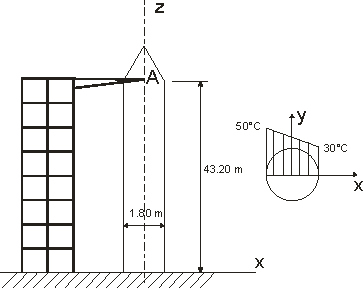
\includegraphics[scale=1.5]{ej4}}
\caption{Torre de lanzamiento de cohetes.}
\label{fig:ej4}
\end{figure}

\textit{Sugerencia:} Calcule la deformación térmica y luego integre para obtener el desplazamiento.\\

\textit{Respuesta}: $10.36[cm]$ 

\dotfill

\begin{quote}
\[
\Delta T>0;\quad \Delta T=|T_{1}-T_{2}|
\]

\[
\mathbf{e}=\alpha\Delta T\mathbf{I} \implies e_{ij}=\alpha\Delta T\delta_{ij}
\]

\[
e_{zz}=\alpha\Delta T=\frac{\partial u_{z}}{\partial z} \implies
du_{z}=\alpha\Delta T\cdot dz
\]

\[
\tan(d\theta)=\theta=\frac{\partial du_{z}}{D}=\frac{\alpha\Delta T}{D}dz
\]

\[
\theta=\int_{0}^{z}d\theta=\int_{0}^{z}\frac{\alpha\Delta T}{D}dz
=\frac{\alpha\Delta T}{D}(z-0)
\]

\[
\theta(z)\approx\tan\theta=\frac{du_{x}}{dz}=\frac{\alpha\Delta T}{D}z
\]

\[
\implies
u_{x}=\int_{0}^{z}\frac{\alpha\Delta T z}{D}dz=\frac{\alpha\Delta T z^{2}}{2D}
=
10^{-5}\left[\frac{1}{\degree C}\right]\cdot
\frac{20[\degree C]}{180[cm]}\cdot
\frac{(4320[cm])^{2}}{2}
=10.368[cm]
\]

\end{quote}

\section*{Ejercicio 5}

Un tubo de acero de longitud 60 cm, diámetro 6 cm, y espesor de pared $\frac{1}{16}$ cm, es estirado axialmente 0.01 cm, expandido 0.001 cm en diámetro y girado en torsión $1\degree$ en su longitud. Determinar las componentes del tensor de deformación.

\textit{Respuesta}:
\[
\begin{array}{cc}
e_{zz}=e_{\theta\theta}=1.66\times 10^{-4}; &
e_{z\theta}= 4.363\times 10^{-4}
\end{array}
\]

\dotfill

\begin{quote}
\begin{align*}
u_{\theta} &= r\frac{\partial\phi}{\partial z}
=r\frac{0.017453}{60[cm]};
&
u_{z} &= \frac{0.01[cm]}{60[cm]}z;
&
u_{r} &= \frac{0.001[cm]}{2}
\end{align*}

\textit{Componentes de deformación infinitesimal en coordenadas polares:}

\begin{align*}
e_{rr} &= \frac{\partial u_{r}}{\partial r}=0                             \\
e_{\theta\theta}
&= \frac{u_{r}}{r}+\frac{1}{r}\frac{\partial u_{\theta}}{\partial \theta}
=\frac{0.001[cm]}{2r}+\frac{1}{r}\cdot 0=\frac{0.001[cm]}{2\cdot 3[cm]}
= 1.6667\times 10^{-4}                                                    \\
e_{r\theta}
&=\frac{1}{2}\left(\frac{1}{r}\frac{\partial u_{r}}{\partial\theta}
+\frac{\partial u_{\theta}}{\partial r}-\frac{u_{\theta}}{r}\right)
=\frac{1}{2}\left(\frac{1}{r}\cdot 0+\phi-\phi\right)=0                   \\
e_{zr} &= \frac{1}{2}\left(\frac{\partial u_{r}}{\partial z}
+\frac{\partial u_{z}}{\partial r}\right)
=\frac{1}{2}(0+0)=0                                                       \\
e_{z\theta} &= \frac{1}{2}\left(\frac{1}{r}
\frac{\partial u_{z}}{\partial\theta}
+\frac{\partial u_{\theta}}{\partial z}\right)
=\frac{1}{2}\left(\frac{1}{r}\cdot 0+r\frac{0.017453}{60[cm]}\right)
=\frac{3[cm]\cdot 0.017453}{2\cdot 60[cm]}=4.3633\times 10^{-4}           \\
e_{zz} &= \frac{\partial u_{z}}{\partial z}=\frac{0.01[cm]}{60[cm]}
=1.6667\times 10^{-4}
\end{align*}
\end{quote}

\section*{Ejercicio 6}

Derive una expresión para el cambio de volumen de un elemento de volumen unitario sometido a deformaciones pequeñas $e_{ij}$. Mostrar que el invariante
$I_{1}=e_{11}+e_{22}+e_{33}$ representa el cambio de volumen por unidad de volumen.

\dotfill

\begin{quote}

\begin{align*}
\mathbf{e} &= \begin{pmatrix}
e_{11} & 0      & 0      \\
0      & e_{22} & 0      \\
0      & 0      & e_{33}
\end{pmatrix} \\ \\
V_{0} &= dS_{0}\cdot dS_{0}\cdot dS_{0} \\
dV &= dS_{1}\cdot dS_{2}\cdot dS_{3} \\ \\
dS_{i}-dS_{0} &= e_{ii}\cdot dS_{0} \\
dS_{i} &= e_{ii}\cdot dS_{0}+dS_{0} \\
dS_{i} &= (e_{ii}+1)dS_{0} \\ \\
V &= (e_{11}+1)dS_{0}\cdot (e_{22}+1)dS_{0}\cdot (e_{33}+1)dS_{0} \\ \\
\lambda &= \frac{V-V_{0}}{V_{0}} \\
&= \frac{[(e_{11}+1)(e_{22}+1)(e_{33}+1)-1]dS_{0}\cdot dS_{0}\cdot dS_{0}}{dS_{0}\cdot dS_{0}\cdot dS_{0}} \\
&= \cancel{1}
+e_{11}+e_{22}+e_{33}
\cancel{+e_{11}e_{22}}
\cancel{+e_{22}e_{33}}
\cancel{+e_{33}e_{11}}
\cancel{+e_{11}e_{22}e_{33}}
\cancel{-1} \\
&= I_{1}
\end{align*}

\end{quote}

\section*{Ejercicio 7}

Sea un dispositivo que permita medir experimentalmente la variación de distancia entre 
dos puntos. Se disponen tres de estos dispositivos en forma de triángulo equilátero como en la figura \ref{fig:ej7}. Dé la expresión del tensor de deformación en la zona, a partir de las medidas de los tres valores de elongación $(\Delta \ell_{12},\Delta \ell_{23},\Delta \ell_{31})$ y de la longitud del lado del triángulo $\ell$.

\begin{figure}[!htbp]
\centerline{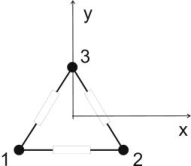
\includegraphics[scale=1.5]{ej7}}
\caption{Disposición de los dispositivos en forma de triángulo}
\label{fig:ej7}
\end{figure}

\dotfill

\begin{quote}

\begin{align*}
e_{11} &= \frac{\partial u_{1}}{\partial x_{1}}=\frac{\Delta l_{12}}{l_{12}} &
e_{1'1'} &= \frac{\partial u_{1'}}{\partial x_{1}'}=\frac{\Delta l_{13}}{l_{13}} &
e_{1''1''} &= \frac{\partial u_{1''}}{\partial x_{1}''}=\frac{\Delta l_{23}}{l_{23}} &
l &= l_{12}=l_{13}=l_{23}
\end{align*}

\begin{align*}
e_{1'1'} &= \frac{e_{11}+e_{22}}{2}
+\frac{e_{11}-e_{22}}{2}\cos{2\alpha}
+\frac{e_{12}}{2}\sin{2\alpha} & \alpha=60\degree \\
&=\frac{\frac{\Delta l_{12}}{l}+e_{22}}{2}
+\frac{\frac{\Delta l_{12}}{l}-e_{22}}{2}\left(-\frac{1}{2}\right)
+\frac{e_{12}}{2}\frac{\sqrt{3}}{2} & (1) \\
e_{1''1''} &= \frac{e_{11}+e_{22}}{2}
+\frac{e_{11}-e_{22}}{2}\cos{2\alpha}
+\frac{e_{12}}{2}\sin{2\alpha} & \alpha=120\degree \\
&=\frac{\frac{\Delta l_{12}}{l}+e_{22}}{2}
+\frac{\frac{\Delta l_{12}}{l}-e_{22}}{2}\left(-\frac{1}{2}\right)
+\frac{e_{12}}{2}\left(-\frac{\sqrt{3}}{2}\right) & (2) \\
(1)-(2): & \\
\frac{\Delta l_{13}}{l}-\frac{\Delta l_{23}}{l} &= \frac{e_{12}}{\sqrt{3}} & \\
e_{12} &= \frac{2}{l\sqrt{3}}(\Delta l_{13}-\Delta l_{23}) & \\
(1)+(2): & \\
\frac{\Delta l_{13}}{l}+\frac{\Delta l_{23}}{l}
&=
\frac{\Delta l_{12}}{l}+e_{22}-\frac{\frac{\Delta l_{12}}{l}-e_{22}}{2} & \\
2\left(\frac{\Delta l_{13}}{l}+\frac{\Delta l_{23}}{l}\right)
&=
\frac{\Delta l_{12}}{l}+2e_{22}+e_{22} & \\
e_{22}
&=
\frac{1}{3}\left(
2\frac{\Delta l_{13}}{l}+2\frac{\Delta l_{23}}{l}-\frac{\Delta l_{12}}{l}
\right) & 
\end{align*}

\end{quote}

\section*{Ejercicio 8}

Dado un campo de tensiones $\sigma_{ij}$, con componentes referidas a un sistema de coordenadas $x_{1},x_{2},x_{3}$:

\begin{enumerate}[a.]
\item ¿Cuál es la definición de tensiones principales?
\item ¿Cuál es la definición de ejes principales?
\item Describir brevemente cómo pueden determinarse, en principio, las direcciones principales (direcciones de los ejes principales).
\item Considere un tensor de deformación $e_{ij}$ referido a los mismos ejes. ¿Cómo determinaría las deformaciones principales y las correspondientes direcciones 
principales de deformación?
\item Si las tensiones y las deformaciones están relacionadas por la expresión
\[
\sigma_{ij}=\lambda e_{kk}\delta_{ij}+2\mu e_{ij}
\]
donde $\lambda,\mu$ son constantes, probar que los ejes principales de tensión coinciden con los ejes principales de deformación.
\end{enumerate}
 
\dotfill

\begin{quote}
\begin{enumerate}[a.]
\item 

Las \textbf{tensiones principales} son los autovalores de $\tau_{ij}$:

\begin{align*}
|\tau_{ij}-\sigma\delta_{ij}| 
&=
\left|\left(\begin{matrix}
\tau_{11} & \tau_{12} & \tau_{13} \\
\tau_{21} & \tau_{22} & \tau_{23} \\
\tau_{31} & \tau_{32} & \tau_{33} \\
\end{matrix}\right)-\sigma
\left(\begin{matrix}
1 & 0 & 0 \\
0 & 1 & 0 \\
0 & 0 & 1 \\
\end{matrix}\right)\right| \\
&=
\left|\begin{matrix}
\tau_{11}-\sigma & \tau_{13} & \tau_{13} \\
\tau_{21} & \tau_{22}-\sigma & \tau_{23} \\
\tau_{31} & \tau_{32} & \tau_{33}-\sigma \\
\end{matrix}\right| \\
&= 
-\sigma^{3}+I_{1}\sigma^{2}-I_{2}\sigma+I_{3} \\
&=
0
\end{align*}

$I_{1}$, $I_{2}$ y $I_{3}$ son invariantes y se calculan de la siguiente manera:

\begin{itemize}
\item \textit{Suma de los elementos de la diagonal: }$I_{1} = \tau_{11}+\tau_{22}+\tau_{33}$

\item \textit{Suma de los determinantes menores que se obtienen de recorrer la diagonal pero sin multiplicar por el pivote: }
\[
I_{2}=
\left|\begin{matrix}
\tau_{22} & \tau_{23} \\
\tau_{32} & \tau_{33} \\
\end{matrix}\right|
+
\left|\begin{matrix}
\tau_{11} & \tau_{13} \\
\tau_{31} & \tau_{33} \\
\end{matrix}\right|
+
\left|\begin{matrix}
\tau_{11} & \tau_{12} \\
\tau_{21} & \tau_{22} \\
\end{matrix}\right|
\]

\item \textit{Determinante de $\tau_{ij}$: }
\[
I_{3}=
\left|
\begin{matrix}
\tau_{11} & \tau_{13} & \tau_{13} \\
\tau_{21} & \tau_{22} & \tau_{23} \\
\tau_{31} & \tau_{32} & \tau_{33} \\
\end{matrix}
\right|
\]
\end{itemize}

\item 

Las \textbf{direcciones principales} son los autovectores de $\tau_{ij}$:

\[
(\tau_{ij}-\sigma\delta_{ij})\cdot\nu_{j}=
\left(\begin{matrix}
\tau_{11}-\sigma & \tau_{13} & \tau_{13} \\
\tau_{21} & \tau_{22}-\sigma & \tau_{23} \\
\tau_{31} & \tau_{32} & \tau_{33}-\sigma \\
\end{matrix}\right)\cdot
\left(\begin{matrix}
\stackrel \sigma \nu_{1} \\
\stackrel \sigma \nu_{2} \\
\stackrel \sigma \nu_{3} \\
\end{matrix}\right)=0
\]

\item Primero se calculan las tensiones principales utilizando lo mostrado en $a$. Luego se calculan las direcciones principales utilizando lo mostrado en $b$.

\item 

Las \textbf{deformaciones principales} son los autovalores de $e_{ij}$:

\begin{align*}
|e_{ij}-e\delta_{ij}| 
&=
\left|\left(\begin{matrix}
e_{11} & e_{12} & e_{13} \\
e_{21} & e_{22} & e_{23} \\
e_{31} & e_{32} & e_{33} \\
\end{matrix}\right)-e
\left(\begin{matrix}
1 & 0 & 0 \\
0 & 1 & 0 \\
0 & 0 & 1 \\
\end{matrix}\right)\right| \\
&=
\left|\begin{matrix}
e_{11}-e & e_{13} & e_{13} \\
e_{21} & e_{22}-e & e_{23} \\
e_{31} & e_{32} & e_{33}-e \\
\end{matrix}\right| \\
&= 
-e^{3}+I_{1}e^{2}-I_{2}e+I_{3} \\
&=
0
\end{align*}

$I_{1}$, $I_{2}$ y $I_{3}$ son invariantes y se calculan de la siguiente manera:

\begin{itemize}
\item \textit{Suma de los elementos de la diagonal: }$I_{1} = e_{11}+e_{22}+e_{33}$

\item \textit{Suma de los determinantes menores que se obtienen de recorrer la diagonal pero sin multiplicar por el pivote: }
\[
I_{2}=
\left|\begin{matrix}
e_{22} & e_{23} \\
e_{32} & e_{33} \\
\end{matrix}\right|
+
\left|\begin{matrix}
e_{11} & e_{13} \\
e_{31} & e_{33} \\
\end{matrix}\right|
+
\left|\begin{matrix}
e_{11} & e_{12} \\
e_{21} & e_{22} \\
\end{matrix}\right|
\]

\item \textit{Determinante de $e_{ij}$: }
\[
I_{3}=
\left|
\begin{matrix}
e_{11} & e_{13} & e_{13} \\
e_{21} & e_{22} & e_{23} \\
e_{31} & e_{32} & e_{33} \\
\end{matrix}
\right|
\]
\end{itemize}

Las \textbf{direcciones principales de deformación} son los autovectores de $e_{ij}$:

\[
(e_{ij}-e\delta_{ij})\cdot\nu_{j}=
\left(\begin{matrix}
e_{11}-e & e_{13} & e_{13} \\
e_{21} & e_{22}-e & e_{23} \\
e_{31} & e_{32} & e_{33}-e \\
\end{matrix}\right)\cdot
\left(\begin{matrix}
\stackrel \sigma \nu_{1} \\
\stackrel \sigma \nu_{2} \\
\stackrel \sigma \nu_{3} \\
\end{matrix}\right)=0
\]

\item 

\begin{align*}
(\sigma_{ij}-\sigma^{\alpha}\delta_{ij})\stackrel{\alpha}{\nu_{j}} &= 0
&
\sigma_{ij} &= \lambda e_{kk}\delta_{ij}+2\mu e_{ij} \\
(\lambda e_{kk}\delta_{ij}
+2\mu e_{ij}
-\sigma^{\alpha}\delta_{ij})
\stackrel{\alpha}{\nu_{j}} &= 0 & \\
(2\mu e_{ij}
+(\lambda e_{kk}-\sigma^{\alpha})\delta_{ij})
\stackrel{\alpha}{\nu_{j}} &= 0 & \\
\left(e_{ij}
+\left(\frac{\lambda e_{kk}-\sigma^{\alpha}\delta_{ij}}{2\mu}\right)\right)
\stackrel{\alpha}{\nu_{j}} &= 0 
& -e^{\alpha}
&=\frac{\lambda e_{kk}-\sigma^{\alpha}\delta_{ij}}{2\mu} \\
(e_{ij}-e^{\alpha}\delta_{ij})\stackrel{\alpha}{\nu_{j}} &= 0 & 
\end{align*}

\end{enumerate}
\end{quote}

\section*{Ejercicio 9}

En un estudio de sismos, Lord Rayleigh propuso una solución de las ecuaciones linealizadas de Elasticidad de la forma:

\[
\begin{array}{l}
u=A\exp(-by+ik(x-ct)) \\
v=B\exp(-by+ik(x-ct)) \\
w=0
\end{array}
\]

Si el plano $xz$ representa la superficie del suelo mientras $y$ representa la profundidad dentro del suelo, y $u,v,w$ representan los desplazamientos de las partículas de suelo, entonces la solución anterior representa una onda propagándose en la dirección $x$ con velocidad $c$ y una amplitud que decrece exponencialmente desde la superficie. Se supone que la onda se generó dentro del suelo y que la superficie del suelo está libre de tensiones.

Después de estudiar las ecuaciones de movimiento y las condiciones de borde, Lord 
Rayleigh halló las constantes $A,B,b$ y $c$, obteniendo:

\[
\begin{array}{l}
u=A(e^{-0.8475ky}-0.5773e^{-0.3933ky})\cos(k(x-C_{R}t))        \\
v=A(-0.8475e^{-0.8475ky}+1.4679e^{-0.3933ky})\sin(k(x-C_{R}t)) \\
w=0
\end{array}
\]
 
La constante $C_{R}$ es llamada velocidad de onda de Rayleigh, y es igual a 0.9174 veces la velocidad de la onda de corte si el coeficiente de Poisson es igual a 0.25. Esta solución satisface las condiciones de una onda propagándose en un medio elástico semi-infinito con superficie libre en $y=0$. Las partículas se mueven en el plano $xy$, con amplitud decreciente a medida que aumenta la distancia a la superficie libre. Esta onda constituye una de las ondas más prominentes que se observan en un sismógrafo 
durante un terremoto.

Responda a las preguntas siguientes, utilizando visualizaciones de los campos de desplazamiento, velocidad y deformación mediante software como Matlab® u $Octave^{(GNU)}$.

\begin{enumerate}[a.]
\item Esquematizar la forma de la onda.
\item Esquematizar la trayectoria de las partículas sobre la superficie libre $y=0$, a 
varios valores de $x$. Repetir para varias partículas a diferentes profundidades $y>0$.
\item Mostrar que el movimiento de las partículas es retrógrado.
\item Determinar la localización y el valor de las máximas deformaciones principales 
a un instante dado.
\end{enumerate}

\dotfill

\begin{quote}

\end{quote}

\section*{Ejercicio 10}

Una membrana cuadrada $(-1\leq x\leq 1,-1\leq y\leq1)$ es estirada de manera que el 
desplazamiento queda descrito por:

\[
\begin{array}{l}
u=a(x^{2}+y^{2}) \\
v=bxy            \\
w=0
\end{array}
\]

\begin{enumerate}[a.]
\item Calcule las componentes de deformación en $(x,y)$.
\item Calcule las deformaciones principales en $(0,0)$.
\end{enumerate}

Asuma que las constantes $a$ y $b$ son mucho menores que 1.

\dotfill

\begin{quote}

\begin{enumerate}[a.]

\item 

\begin{align*}
x &= 1-(-1)=2 \\
y &= 1-(-1)=2 \\
e_{11} &= \frac{1}{2}
\left(
\frac{\partial u_{1}}{\partial x_{1}}+\frac{\partial u_{1}}{\partial x_{1}}
\right)
= \frac{\partial u_{1}}{\partial x_{1}}=\frac{\partial u}{\partial x}=2ax & \\
e_{22} &= \frac{1}{2}
\left(
\frac{\partial u_{2}}{\partial x_{2}}+\frac{\partial u_{2}}{\partial x_{2}}
\right)
= \frac{\partial u_{2}}{\partial x_{2}}=\frac{\partial v}{\partial y}=bx & \\
e_{12} &= \frac{1}{2}
\left(
\frac{\partial u_{2}}{\partial x_{1}}+\frac{\partial u_{1}}{\partial x_{2}}
\right)
= \frac{1}{2}\left(
\frac{\partial v}{\partial x}+\frac{\partial u}{\partial y}\right) 
=\frac{1}{2}(by+2ay) \\ 
\mathbf{e} &= \begin{pmatrix}
2ax                 & \frac{1}{2}(by+2ay) \\
\frac{1}{2}(by+2ay) & bx
\end{pmatrix} \\
\end{align*}

\item 

\begin{align*}
(e_{1},e_{2}) &= \frac{e_{x}+e_{y}}{2}\pm
\sqrt{\left(\frac{e_{x}-e_{y}}{2}\right)^{2}+e_{xy}^{2}} \\
&= (0,0)
\end{align*}

\end{enumerate}

\end{quote} 

\section*{Apéndice}

\textit{Relación de estiramiento:}

\begin{equation}
\lambda=\frac{\text{Longitud deformada}}{\text{Longitud original}}=\frac{L}{L_{0}}
\end{equation}

\textit{Coordenadas de una partícula en la configuración original del cuerpo:}

\[
(a_{1},a_{2},a_{3})
\]

\textit{Coordenadas de una partícula en la configuración deformada del cuerpo:}

\[
(x_{1},x_{2},x_{3})
\]

\textit{La configuración en un sistema se puede determinar en función de la configuración en el otro sistema:}

\begin{equation}
x_{i}=x_{i}(a_{1},a_{2},a_{3})=
\begin{pmatrix}
x_{1}(a_{1},a_{2},a_{3}) \\
x_{2}(a_{1},a_{2},a_{3}) \\
x_{3}(a_{1},a_{2},a_{3})
\end{pmatrix}
\end{equation}

\begin{equation}
a_{i}=a_{i}(x_{1},x_{2},x_{3})=
\begin{pmatrix}
a_{1}(x_{1},x_{2},x_{3}) \\
a_{2}(x_{1},x_{2},x_{3}) \\
a_{3}(x_{1},x_{2},x_{3})
\end{pmatrix}
\end{equation}

\textit{Vector desplazamiento $\mathbf{u}$:}

\begin{equation}
u_{i}=x_{i}-a_{i}
\end{equation}

\textit{Vector desplazamiento en función de la posición original: (Para sólidos, enfoque Lagrangiano)}

\begin{equation}
u_{i}(a_{1},a_{2},a_{3})=x_{i}(a_{1},a_{2},a_{3})-a_{i}
\end{equation}

\textit{Vector desplazamiento en función de la posición deformada: (Para fluidos, enfoque Euleriano)}

\begin{equation}
u_{i}(x_{1},x_{2},x_{3})=x_{i}-a_{i}(x_{1},x_{2},x_{3})
\end{equation}

\textit{Deformation vs Strain:}

\begin{center}
deformation $\implies$ movimiento, traslación \\
strain $\implies$ deformación
\end{center}

\textit{Descripción del cambio entre dos puntos:}

\begin{eqnarray}
Lagrangiano: & ds_{0}^{2}=da_{1}^{2}+da_{2}^{2}+da_{3}^{2} \\
             &                                   \nonumber \\
Euleriano:   & ds^{2}=dx_{1}^{2}+dx_{2}^{2}+dx_{3}^{2}
\end{eqnarray}

\textit{Tensor de deformación de Green (Lagrangiano):}

\begin{equation}
E_{ij}=\frac{1}{2}\left(
\delta_{\alpha\beta}
\frac{\partial x_{\alpha}}{\partial a_{i}}
\frac{\partial x_{\beta}}{\partial a_{j}}-\delta_{ij}
\right)
=
\frac{1}{2}\left(
\frac{\partial x_{\alpha}}{\partial a_{i}}
\frac{\partial x_{\alpha}}{\partial a_{j}}-\delta_{ij}
\right)
=
\frac{1}{2}\left(
\frac{\partial x_{\beta}}{\partial a_{i}}
\frac{\partial x_{\beta}}{\partial a_{j}}-\delta_{ij}
\right)=E_{ji}
\end{equation}

\begin{equation}
dS^{2}-dS_{0}^{2}=2E_{ij}da_{i}da_{j}
\end{equation}

\textit{Tensor de deformación de Almansi (Euleriano):}

\begin{equation}
e_{ij}=\frac{1}{2}\left(
\delta_{ij}-
\delta_{\alpha\beta}
\frac{\partial a_{\alpha}}{\partial x_{i}}
\frac{\partial a_{\beta}}{\partial x_{j}}
\right)
=
\frac{1}{2}\left(
\delta_{ij}-
\frac{\partial a_{\alpha}}{\partial x_{i}}
\frac{\partial a_{\alpha}}{\partial x_{j}}
\right)
=
\frac{1}{2}\left(
\delta_{ij}-
\frac{\partial a_{\beta}}{\partial x_{i}}
\frac{\partial a_{\beta}}{\partial x_{j}}
\right)=e_{ji}
\end{equation}

\begin{equation}
dS^{2}-dS_{0}^{2}=2e_{ij}dx_{i}dx_{j}
\end{equation}

\textit{Tensor de deformación infinitesimal de Cauchy: (Lagrangiano = Euleriano)}

\begin{equation}
e_{ij}=\frac{1}{2}\left(
\frac{\partial u_{j}}{\partial x_{i}}+
\frac{\partial u_{i}}{\partial x_{j}}
\right)
=
\frac{1}{2}\left(
\frac{\partial u_{j}}{\partial a_{i}}+
\frac{\partial u_{i}}{\partial a_{j}}
\right)
\end{equation}

\begin{equation}
dS^{2}-dS_{0}^{2}=2e_{ij}dx_{i}dx_{j}=2e_{ij}da_{i}da_{j}
\end{equation}

\textit{Componentes de deformación infinitesimal en coordenadas polares:}

\begin{equation}
\begin{array}{l}
\displaystyle e_{rr}=\frac{\partial u_{r}}{\partial r}                  \\ \\
\displaystyle e_{\theta\theta}
=\frac{u_{r}}{r}+\frac{1}{r}\frac{\partial u_{\theta}}{\partial \theta} \\ \\
\displaystyle e_{r\theta}
=\frac{1}{2}\left(\frac{1}{r}\frac{\partial u_{r}}{\partial\theta}
+\frac{\partial u_{\theta}}{\partial r}-\frac{u_{\theta}}{r}\right)     \\ \\
\displaystyle e_{zr}=\frac{1}{2}\left(\frac{\partial u_{r}}{\partial z}
+\frac{\partial u_{z}}{\partial r}\right)                               \\ \\
\displaystyle e_{z\theta}=\frac{1}{2}\left(\frac{1}{r}
\frac{\partial u_{z}}{\partial\theta}
+\frac{\partial u_{\theta}}{\partial z}\right)                          \\ \\
\displaystyle e_{zz}=\frac{\partial u_{z}}{\partial z}
\end{array}
\end{equation}

\textit{Tensor de rotación infinitesimal:}

\begin{equation}
\omega_{ij}=\frac{1}{2}\left(
\frac{\partial u_{j}}{\partial x_{i}}-
\frac{\partial u_{i}}{\partial x_{j}}
\right)
=
\begin{pmatrix}
0            & \omega_{12}  & -\omega_{13} \\
-\omega_{12} & 0            & \omega_{23}  \\
\omega_{31}  & -\omega_{23} & 0
\end{pmatrix}
=-\omega_{ji};
\quad \mbox{Antisimétrico}
\end{equation}

\textit{Vector dual de rotación infinitesimal:}\\

\begin{minipage}{0.3\linewidth}

\begin{equation}
\omega_{k}=\frac{1}{2}\varepsilon_{kij}\omega_{ij}
\end{equation}

\end{minipage} \hfill \begin{minipage}{0.3\linewidth}

Se llama vector dual porque a partir de él se puede determinar el tensor de rotación infinitesimal y viceversa:

\end{minipage} \hfill \begin{minipage}{0.3\linewidth}

\begin{equation}
\omega_{ij}=\varepsilon_{ijk}\omega_{k}
\end{equation}

\end{minipage}\\

\textit{Deformaciones principales:}

\begin{equation}
|e_{ij}-e\delta_{ij}|=0
\end{equation}

\textit{Direcciones principales de deformación:}

\begin{equation}
(e_{ij}-e_{p}\delta_{ij})\stackrel{p}{\nu_{j}}=0;\quad p=1,2,3
\end{equation}

\begin{thebibliography}{1}
\bibitem{MCF}
Y. C. Fung,
\emph{A First Course in Continuum Mechanics}, 
tercera edición,
PRENTICE HALL,
1994.
\end{thebibliography}

\end{document}